\section{R18: matched satellite forecasts with Orekit}
\label{sec:r18-orbit-comparison}

\begin{panel}
The new comparison establishes close numerical agreement with an independent
Orekit implementation of the same frozen orbital problem. It does not establish
better satellite-position accuracy than Orekit. Across eight cases, the maximum
aTOMos CPU--Orekit position difference is $0.026760$\,m and the maximum
CPU--CUDA difference is $0.000220015$\,m. Both engines show almost the same
discrepancies against later external positions: all eight first-day sampled
maxima are below $10$\,m, while some seven-day maxima reach kilometres.
\end{panel}

\subsection{The physical problem and observations are matched}
The retained ORBIT-DYNAMICS-R2 models are evaluated for G05 (MEO), C03 (GEO),
C06 (IGSO) and CHANDRA (HEO), from the 2 January and 2 February 2025 GPST
epochs. The original models, training provenance, reference products, native
binaries and scorer sources were frozen under 71 input hashes before these
R18 numerical comparisons. No target-position fit, clock adjustment, frame
alignment or physical parameter selection is performed here. Both date sets
were already inspected in R10; neither is a newly blind R18 confirmation.

Each implementation receives the same initial six-state vector, degree/order
12 EGM96 coefficients, Sun/Moon forcing series, solar-pressure and cylindrical
shadow rule, empirical RTN acceleration, relativity setting and frame series.
Orekit 13.1.8 with Hipparchus 4.0.3 supplies its numerical propagator,
Holmes--Featherstone gravity algorithm and relativity implementation. Independent
Java adapters preserve the other frozen force equations. Orekit's normalized
gravity coefficients are converted from the same frozen unnormalized table.
Its central term is added once, with automatic central attraction disabled.
The final adapter uses absolute Cartesian position/velocity states and
explicitly checks short-time motion; no orbit determination is performed.

The upstream \href{https://www.orekit.org/static/apidocs/org/orekit/propagation/numerical/NumericalPropagator.html}{numerical-propagator API}
describes configurable integration and force models; the
\href{https://www.orekit.org/static/apidocs/org/orekit/forces/gravity/HolmesFeatherstoneAttractionModel.html}{Holmes--Featherstone API}
describes normalized coefficients and its stable gravity recurrence. The actual
13.1.8 binary and source archive are separately pinned in
\path{review/r18_orbit_java_dependencies.json}; the live documentation links
are explanatory references, not the version pin.

For GNSS, the independent SP3 parser retains the original GBM precise positions
and their IGS20/IGb20 realization labels. Both engines use the same frozen
GCRS-to-ECEF transform for scoring. CHANDRA uses the original Horizons
geometric geocentric ICRF table, with calendar TDB converted to GPST through
SOFA/ERFA. Each returned epoch must equal the exact decoded request epoch;
all 15,553 rows match with zero engine/request timestamp offset. This checks
alignment of the calculation, not the accuracy of a live clock.

Seven cases contain 2,016 future samples. February C03 contains 1,441 and has
a $172800$\,s reference gap. Missing rows are not filled. CHANDRA's final
samples lie about $51.184$\,s before the nominal seven-day GPST endpoint;
the files retain exact horizon offsets. Every first-day statistic below uses
288 available samples. Full reports also contain cumulative 1, 6, 12, 48 and
72 hour statistics, first sampled threshold exceedances and reference gaps.

\subsection{Physical-reference discrepancy remains horizon dependent}
For common reference position $r_i$ and engine position $p_i^a$ in the declared
comparison frame, the measured quantities are
\begin{equation}
 e_i^a=\lVert p_i^a-r_i\rVert_2,\qquad
 E_{\mathrm{RMS}}^a=\sqrt{\frac{1}{N}\sum_{i=1}^{N}(e_i^a)^2},\qquad
 E_{\max}^a=\max_i e_i^a.
\end{equation}
Table~\ref{tab:r18-orbit-errors} reports metres, rounded to three decimals.
``Arc'' means all available future samples up to seven days; it is not a
continuous-time bound. CUDA is omitted from this compact physical-error table
because its separate maximum state disagreement with CPU is quantified in
Table~\ref{tab:r18-orbit-numerics}; its complete scores remain in the JSON report.

\begin{table}[htbp]
\centering\small\setlength{\tabcolsep}{3pt}
\begin{tabular}{llrrrrrr}
\toprule
 & & \multicolumn{2}{c}{0--24 h maximum} & \multicolumn{2}{c}{Arc maximum} & \multicolumn{2}{c}{Arc RMS}\\
Epoch & Object & CPU & Orekit & CPU & Orekit & CPU & Orekit\\
\midrule
Jan & G05 & 1.057 & 1.056 & 12.998 & 12.975 & 5.294 & 5.281\\
Jan & C03 & 5.304 & 5.304 & 78.717 & 78.716 & 37.434 & 37.434\\
Jan & C06 & 1.172 & 1.172 & 8.084 & 8.083 & 2.943 & 2.943\\
Jan & CHANDRA & 8.093 & 8.093 & 25635.951 & 25635.961 & 5412.235 & 5412.237\\
Feb & G05 & 3.072 & 3.069 & 71.800 & 71.773 & 33.113 & 33.099\\
Feb & C03 & 4.654 & 4.654 & 100604.174 & 100604.175 & 39382.862 & 39382.863\\
Feb & C06 & 2.108 & 2.108 & 7.629 & 7.630 & 3.494 & 3.494\\
Feb & CHANDRA & 0.290 & 0.290 & 5663.182 & 5663.184 & 2055.685 & 2055.685\\
\bottomrule
\end{tabular}
\caption{Matched forecast discrepancy against later GBM/Horizons positions,
in metres. Both engines solve the same frozen physical model.}
\label{tab:r18-orbit-errors}
\end{table}

The first-day maxima span $0.289813$--$8.092836$\,m for native CPU. G05's
seven-day maxima are $12.998$ and $71.800$\,m; C06's are $8.084$ and
$7.629$\,m. The larger discrepancies must remain visible: January CHANDRA
reaches $25.636$\,km, February CHANDRA $5.663$\,km and February C03
$100.604$\,km. Closely matching these curves in Orekit shows that a different
integrator alone does not remove the long-horizon discrepancy. This experiment
does not uniquely separate force-model limitations, unmodelled events and
reference-data limitations, and does not infer a cause from a plotted jump.

\subsection{Numerical agreement is a separate measurement}
Define the same-epoch state-position difference
$d_i^{a,b}=\lVert x_i^a[0{:}3]-x_i^b[0{:}3]\rVert_2$ in the common inertial
coordinates. Standard Orekit integration uses a $10^{-6}$\,m positional
absolute tolerance and a 60\,s maximum step; refinement uses $10^{-7}$\,m
and 15\,s. Velocity absolute tolerances are respectively $10^{-9}$ and
$10^{-10}$\,m/s, with relative tolerance $2\times10^{-14}$. These are
integrator controls, not certified physical-position tolerances.

\begin{table}[htbp]
\centering\small\setlength{\tabcolsep}{5pt}
\begin{tabular}{llrrrr}
\toprule
 & & \multicolumn{4}{c}{Maximum state-position difference (mm)}\\
Epoch & Object & CPU--CUDA & CPU--Orekit & CUDA--Orekit & Orekit refinement\\
\midrule
Jan & G05 & 0.043202 & 26.652946 & 26.696136 & 0.026221\\
Jan & C03 & 0.040229 & 1.035783 & 0.995845 & 0.011058\\
Jan & C06 & 0.014359 & 1.081491 & 1.095529 & 0.021503\\
Jan & CHANDRA & 0.019398 & 9.973403 & 9.992799 & 0.064834\\
Feb & G05 & 0.027756 & 26.759896 & 26.786545 & 0.018755\\
Feb & C03 & 0.024485 & 1.027233 & 1.050839 & 0.006472\\
Feb & C06 & 0.005661 & 1.009391 & 1.013778 & 0.027620\\
Feb & CHANDRA & 0.220015 & 6.077876 & 6.297885 & 0.022174\\
\bottomrule
\end{tabular}
\caption{Numerical disagreement over each complete sampled arc. Orekit columns
use the standard run; refinement compares its standard and tighter controls.}
\label{tab:r18-orbit-numerics}
\end{table}

The maximum Orekit refinement displacement is $0.064834$\,mm, occurring in
January CHANDRA; the GNSS maximum is $0.027620$\,mm. An independent force
audit evaluates 65 points on each standard trajectory against the retained
Python R2 equations: 520 checks, with maximum acceleration discrepancy
$1.115761\times10^{-15}$\,m/s$^2$. The completed audit binds the exact final
adapter, dependency manifest, requests and all 16 standard/refined state files.
The tight run is scored against the same external rows in a second full report.

These results make the numerical contribution small compared with the measured
metre-to-kilometre reference discrepancies in this experiment. They do not make
the arithmetic exact. Lossless one-bit word packing preserves the encoded model
and operators; native physical propagation still uses finite-precision
floating-point arithmetic. The discrete exactness proofs elsewhere in this
document and the numerical orbital agreement above are different guarantees.

\subsection{Reference checks, runtime scope and reproducibility}
The independent GBM/WUM product intersection yields seven-day RMS discrepancies
of $0.02436/0.02447$\,m for G05, $0.16894/0.15315$\,m for C06 and
$2.20440/0.93894$\,m for C03 (January/February). The largest C03 product
discrepancy is $3.57510$\,m in January. These are observed cross-product
differences, not a certified uncertainty floor; providers can share observations
and modelling assumptions. CHANDRA has no second trajectory product in this
experiment. The common frozen EOP transform and the GCRS/ICRF coordinate
approximation remain stated limitations, as does retrospective product
availability. Correlated sampled positions supply no general confidence level.

Native one-batch durations include worker startup, model initialization, query
execution and teardown. CPU takes about $0.43$--$0.57$\,s for the GNSS cases
and $2.23$\,s for CHANDRA; CUDA takes $21.2$--$24.0$\,s and
$84.6$--$87.5$\,s respectively. These single trials are diagnostic, and show
no GPU advantage for this particular workload and lifecycle. Orekit's reported
internal timing has a different boundary, so no cross-library speed ratio is
claimed. The finite-word spatial and journal benchmarks retain their separate
workloads and cannot substitute for this orbit comparison.

\path{formal/ORBIT_COMPARISON_PROTOCOL.md} states the frozen experiment;
\path{formal/ORBIT_COMPARISON_RESULTS.md} records the results and exact hashes.
The scoring script is \path{tools/compare_orbit_references.py}. Its standard and
tight summaries are \path{review/orbit_comparison/matched_forecast_summary.json}
and \path{review/orbit_comparison/matched_forecast_tight_summary.json}.
The numerical admission record is \path{review/r18_orekit_numerical_audit.json}.
Plot generation verifies these bindings and recomputes the displayed errors
from the frozen reference rows and scored states.

NASA describes \href{https://naif.jpl.nasa.gov/naif/index.html}{SPICE as an
observation-geometry system}. Its separate SPK interpolation experiment in this
release measures representation of a supplied frozen forecast. Neither that
experiment nor the matched Orekit calculation establishes universal superiority
over a space agency's navigation system. What this adds is a reproducible
external numerical comparison and explicit accuracy-versus-horizon evidence for
the existing seeds.

\begin{figure}[p]
\centering
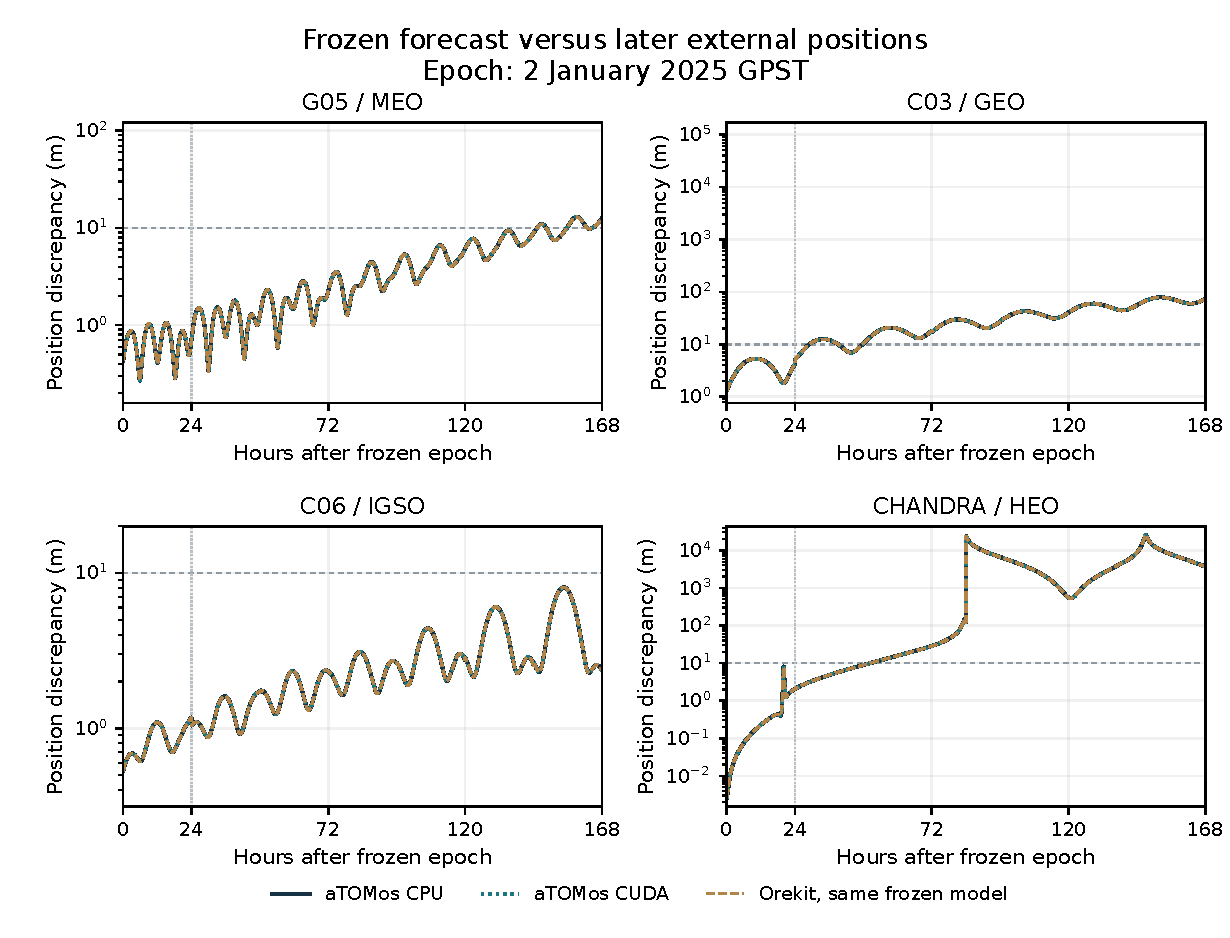
\includegraphics[width=\textwidth]{figures/r18_orbit_forecast_jan.pdf}
\caption{January forecast discrepancies. Curves from the three implementations
nearly overlap. The horizontal 10\,m line is descriptive; the vertical dotted
line marks 24 hours. Per-object vertical scales match the February panels.
Selected sampled error is shown, with no reference-derived alignment.}
\label{fig:r18-orbit-jan}
\end{figure}
\begin{figure}[p]
\centering
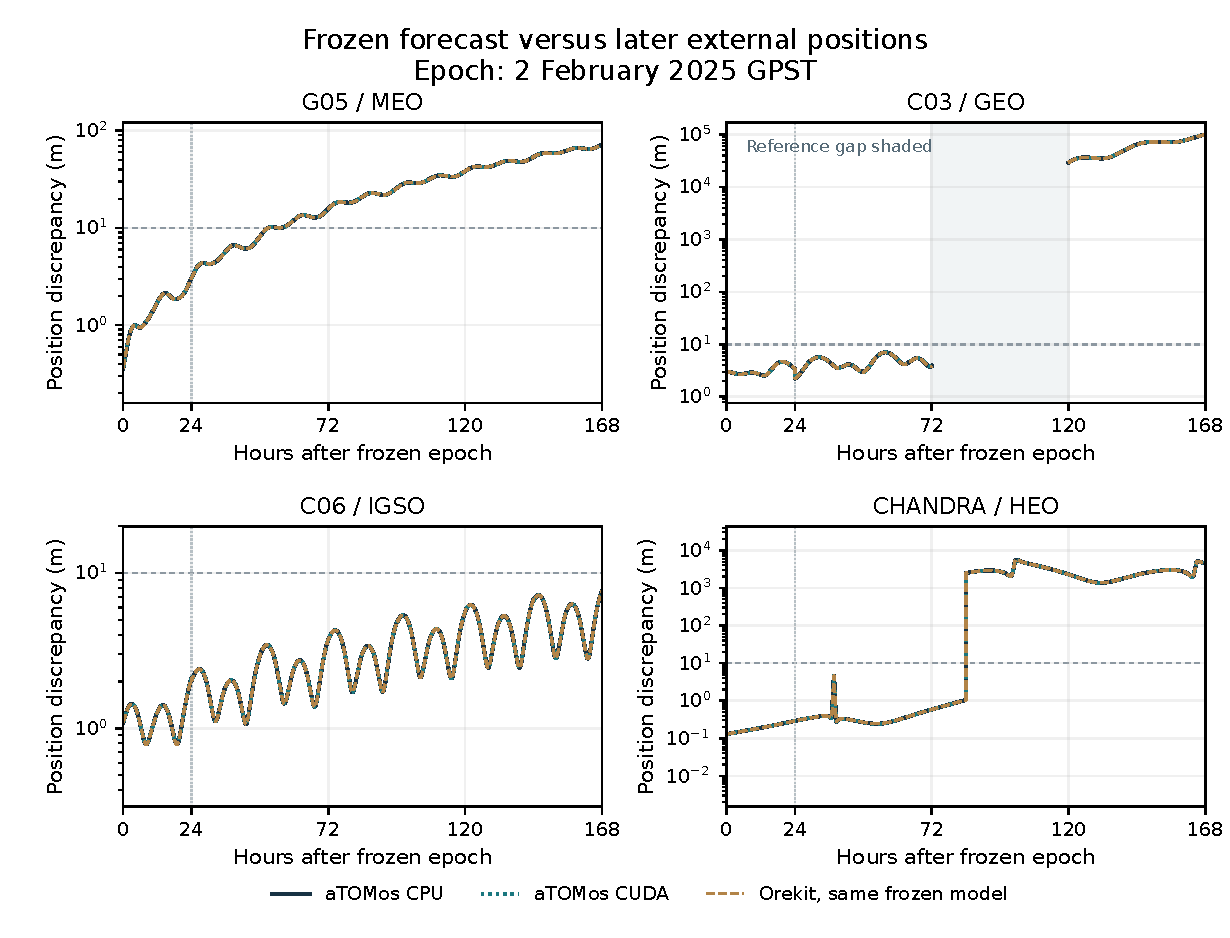
\includegraphics[width=\textwidth]{figures/r18_orbit_forecast_feb.pdf}
\caption{February forecast discrepancies. The missing two-day C03 reference arc
is shaded and the curves are broken there. Sparse or absent observations do not
establish performance between the retained samples.}
\label{fig:r18-orbit-feb}
\end{figure}
\clearpage
